\subsubsection{Purpose}
This sub-part of the "Use Car" functionality focuses on the sequence of sub-functionalities involved in the car unlocking process.

The purpose of the functionality is that of allowing the user to unlock the car he/she reserved based on his/her actual proximity to the vehicle - given the GPS of a mobile device is available - or upon the insertion of a vehicle-specific code into the application.

\subsubsection{Scenario 1}
Damian reserved a \emph{PowerEnJoy} car and is walking towards the vehicle location. When he reaches the car, he takes out his smartphone and opens the \emph{"Reserve Car"} function of the mobile app. The system shows the current reservation: since Damian is close enough to the car and the GPS is active on his mobile device, the \emph{"Unlock car"} button has been activated. He taps on the button and the car unlocks, enabling him to enter it.

\subsubsection{Scenario 2}
Elsa stayed out later than usual to study for her exams, and decided to rent a \emph{PowerEnJoy} car with her laptop. Her smartphone has low battery, so she decided to turn the GPS off to make the battery last longer. Once she gets to the car, she tries to unlock it by making the system detect her proximity. Since the button does not activate, she remembers that the GPS is off and decides to input the car code into the mobile app; she then finds the dedicated car code, opens the right function by tapping on the \emph{"Unlock with car code"} button and inputs it. The system processes the request and, having verified that the user who inserted the code is the same who reserved the car, properly unlocks the vehicle and lets Elsa enter it.

\subsubsection{Use-case}
A detail of the use-case is provided in Table \ref{unlock_car_uc}

\subsubsection{Functional requirements}
\begin{enumerate}
\item Upon every try, the system must check that the user trying to unlock the car is the same that reserved it;
\item The system must guarantee to recognize the proximity of the user if he/she is within a 2 m radius from the car and has the GPS active on a mobile device;
\item The system must always guarantee the possibility for the user to unlock the vehicle he/she reserved by inserting the car code instead of using the GPS proximity detection system;
\item Upon every code insertion, the system must check that the code is the one associated with the car reserved by the user who inserted the code;
\item The vehicle-specific code must be unique for each car.
\item The reservation expiration timer must stop as soon as the car is unlocked;
\end{enumerate}

\begin{table}[H]
\begin{center}
\begin{tabular}{p{0.3\textwidth} | p{0.7\textwidth}}
\hline
Actor & Logged user\\
\hline
Goal & Goal 5\\
\hline
Input Condition & The user reserved a car and is in its proximity OR The user reserved a car inserted the car code into the application\\
\hline
Event Flow & 
\begin{enumerate}
\item The user who reserved the vehicle approaches it and opens the mobile application;
\item The user opens the \emph{"Reserve car"} function and the system provides the sum-up of his/her active reservation;
\item The user either: has the GPS active and taps onto the \emph{"Unlock car"} button OR reads and inserts the car code into the application, tapping the \emph{"Unlock with car code"} button;
\item The system processes the request, by verifying that the user who tries to unlock the car is the one who reserved it;
\item The system unlocks the vehicle.
\end{enumerate} \\
\hline
Output Condition & The car is unlocked and the user can access it.\\
\hline
Exception & If the user wants to unlock the car but he/she is further than 2 m away from it, the \emph{"Unlock car"} button on the reservation screen will not be active.

If the user inputs a wrong code when trying to unlock the car, the system will notify that the code is wrong and will not unlock the car, sending the user back to the reservation page on the application.\\
\hline
\end{tabular}
\end{center}
\caption{Unlock car use-case}
\label{unlock_car_uc}
\end{table}

\begin{figure}[H]
\begin{center}
		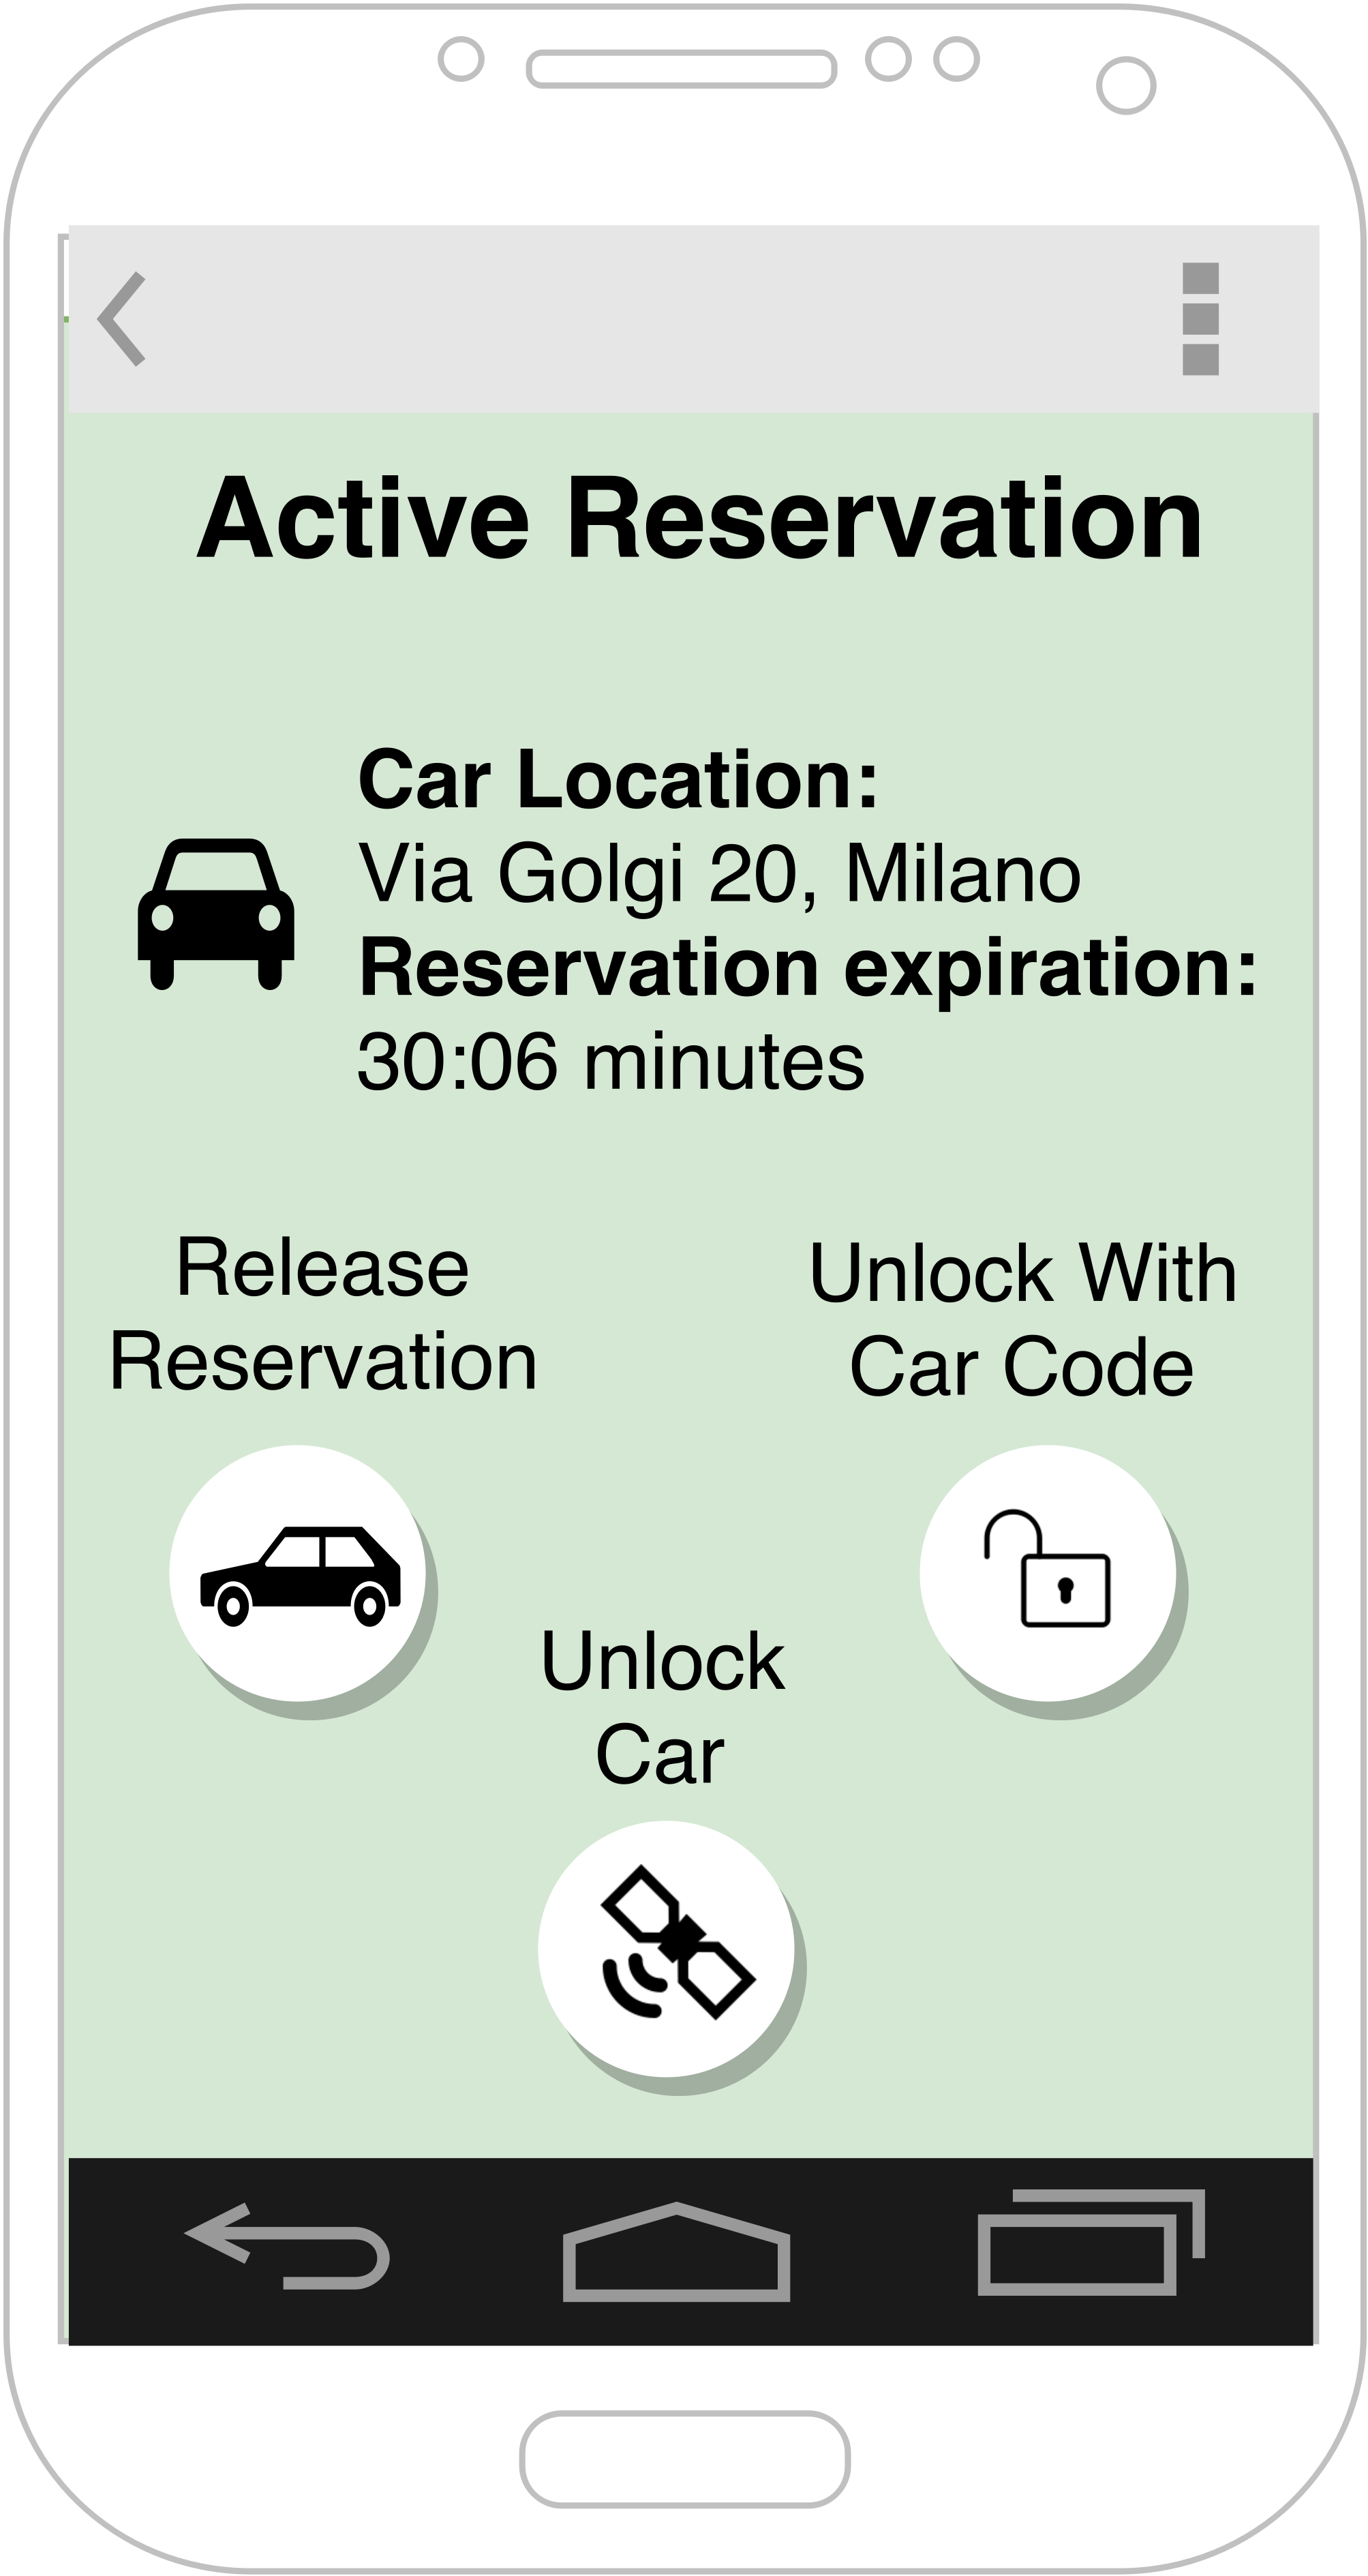
\includegraphics[width=0.4\textwidth]{./specific_requirements/features/diagrams/mobile_unlock.png}
		\caption{Mockup of the mobile unlock feature accessible from the reservation screen.}
		\label{mobile_unlock}
\end{center}
\end{figure}